\PassOptionsToPackage{table}{xcolor}
\documentclass[aspectratio=169]{beamer}
\hypersetup{pdfpagemode=FullScreen}
\usepackage[utf8]{inputenc}
\usepackage[T1]{fontenc}
\usepackage{lmodern}
\usepackage[english]{babel}
\usepackage{graphicx}
\usepackage{amsmath}
\usepackage{amsfonts}
\usepackage{amssymb}
%\usetheme{CambridgeUS}
%\usepackage[table,xcdraw]{xcolor}
\usepackage{pgfgantt}
%\usetheme{Berlin}
%\usetheme{Montpellier}
\usetheme{Boadilla}
\useinnertheme{circles}
\renewcommand{\footnotesize}{\fontsize{6pt}{10pt}\selectfont}
%\usepackage[nottoc]{tocbibind}
\usepackage{cite}
%\useoutertheme{miniframes} % Alternatively: miniframes, infolines, split
%\useinnertheme{circles}
%\usecolortheme{default}
%\usecolortheme{dolphin}
\usepackage{hyperref}
\usefonttheme[onlymath]{serif}
\setbeamertemplate{caption}[numbered]
\setbeamertemplate{bibliography item}{\insertbiblabel}
%\hypersetup{
	%	colorlinks=true,
	%	linkcolor=blue,
	%	filecolor=magenta,      
	%	urlcolor=cyan,
	%}
\renewcommand{\figurename}{Fig.}
\setbeamertemplate{section in toc}[sections numbered]
\insertsectionnavigationhorizontal{.5\textwidth}{\hskip0pt plus1filll}{}
%\setbeamertemplate{frametitle}[rounded]
\setbeamertemplate{blocks}[rounded][shadow]



\defbeamertemplate*{footline}{CambridgeUS theme}
{
	\leavevmode%
	\hbox{%
		\begin{beamercolorbox}[wd=.333333\paperwidth,ht=2.25ex,dp=1ex,center]{author in head/foot}%
			\usebeamerfont{author in head/foot}%\insertshortauthor
			~~\insertshortinstitute
		\end{beamercolorbox}%
		\begin{beamercolorbox}[wd=.333333\paperwidth,ht=2.25ex,dp=1ex,center]{title in head/foot}%
			\usebeamerfont{title in head/foot}\insertshorttitle
		\end{beamercolorbox}%
		\begin{beamercolorbox}[wd=.333333\paperwidth,ht=2.25ex,dp=1ex,right]{date in head/foot}%
			\usebeamerfont{date in head/foot}\hspace*{2em}
			Slide: \insertframenumber{} of \inserttotalframenumber\hspace*{2ex}
	\end{beamercolorbox}}%
	\vskip0pt%
}



\defbeamertemplate*{headline}{CambridgeUS theme}
{
	\leavevmode%
	\hbox{%
		\begin{beamercolorbox}[wd=.333333\paperwidth,ht=2.25ex,dp=1ex,center]{author in head/foot}%
			\usebeamerfont{author in head/foot}%\insertshortauthor
			~~%\insertshortinstitute
		\end{beamercolorbox}%
		\begin{beamercolorbox}[wd=.333333\paperwidth,ht=2.25ex,dp=1ex,center]{title in head/foot}%
			\usebeamerfont{title in head/foot}%\insertshorttitle
		\end{beamercolorbox}%
		\begin{beamercolorbox}[wd=.333333\paperwidth,ht=2.25ex,dp=1ex,right]{date in head/foot}%
			\usebeamerfont{date in head/foot}\insertshortdate{}\hspace*{2em}
			\textsl{\emph{{{{\tiny {\tiny }}}}}}%\insertframenumber{} of \inserttotalframenumber\hspace*{2ex}
	\end{beamercolorbox}}%
	\vskip0pt%
}



\definecolor{UniBlue}{RGB}{83,121,170}

\setbeamercolor{title}{fg=white, bg=UniBlue}
%\setbeamercolor{title in head/foot}{fg=black,bg=lightgray}
%\setbeamercolor{author in head/foot}{fg=white,bg=black}
%\setbeamercolor{frametitle}{fg=white,bg=black}
%\setbeamercolor{block title}{fg=white,bg=black}
%\setbeamercolor{block body}{bg=lightgray, fg=black}
%\setbeamercolor{date in head/foot}{fg=white, bg=black}
%\setbeamercolor{item}{fg=gray}






\begin{document}
	%\author{}
	\title{Power Distribution System for a CubeSat}
	
	\subtitle{}
	%\logo{}
	
	
	\author{Presented by :\\Ansaf Niyaz | TRV19EE016  \and Govind Murali | TRV19EE025  \and \\Jijesh J. Kumar | TRV19EE029  \and Naveen A.B. | TRV19EE038}
	
	\institute{GEC Barton Hill,Thiruvananthapuram}
	\date{\today}
	
	
	\setbeamercovered{transparent}
	\setbeamertemplate{navigation symbols}
	{%
		\hbox{%
			\hbox{\insertslidenavigationsymbol}
			\hbox{\insertframenavigationsymbol}
			\hbox{\insertsubsectionnavigationsymbol}
			\hbox{\insertsectionnavigationsymbol}
			\hbox{\insertdocnavigationsymbol}
			\hbox{\insertbackfindforwardnavigationsymbol}}%
	}
	\begin{frame}[plain]
		\maketitle
		\center{Guided by: Prof. Dinesh Gopinath}
		%	\center{{SEMINAR PRESENTATION}}
	\end{frame}
	
	
	\begin{frame}
		\frametitle{Contents}
		
		
		
		
		\tableofcontents
	\end{frame}
	
	
	
	\section{Objectives}
	\begin{frame}
		
		\frametitle{Objective}
		To design and implement a fully autonomous power generation, storage and distribution system for a CubeSat 
		
		
		
	\end{frame}
	
	
	
	
	\section{Project Outline}
	
	\begin{frame}
		\frametitle{Project Outline	}
		
		\begin{minipage}{0.5\textwidth}
			CubeSat (1U):
			\begin{itemize}
				
				\item Dimensions - 10x10x10 $cm^{3} $
				\item Weight - 2 kg.
			\end{itemize}
		\end{minipage}
		\begin{minipage}{0.3\textwidth}
			\begin{figure}
				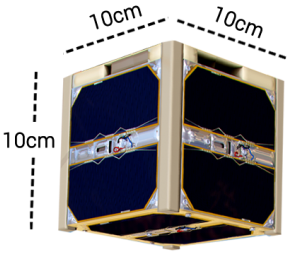
\includegraphics[width=5.1cm]{cubes1.png}
				\begin{center}
					\caption{CubeSat 1U (Source: GIS Geography )}
				\end{center}
				\label{fig:trac2}
				
			\end{figure}
			
		\end{minipage}
		
	\end{frame}

	
	\begin{frame}
		\frametitle{Project Outline (Contd.)}
		Electrical Power System (EPS):
		\begin{itemize}
			
			\item Harvests energy from the solar panels
			\item Manages power storage and distribution
			\item Protects circuits from damage
			\item Redundant architecture
		\end{itemize}
	\end{frame}
	
	
		\section{Literature Review}
		\begin{frame}
		\frametitle{Literature Review}

				
			Power Generation and Storage:
			\begin{itemize}
			\item  Solar cells and batteries used for generation and storage of power respectively
			\item Batteries supply power during absence of solar energy
			\item Li-ion batteries are preferred to Ni-MH\cite{p4}
		\end{itemize}
	
	
		Power Conditioning:
	\begin{itemize}
		\item DC-DC converters are preferred to linear voltage regulators to reduce losses
		\item Peak power transfer is preferred to direct power transfer for solar output\cite{p2}
		\item Trickle charge\cite{p3} method is used to charge the batteries
		\item 5V and 3.3V DC-DC convertors outputs regulated voltage to their respective DC	 buses
	\end{itemize}
	\end{frame}
	\begin{frame}
		\frametitle{Literature Review (Contd.)}
		
				Power Distribution:
		\begin{itemize}
			\item Distributed EPS scheme\cite{p1} is preferred to increase flexibility
			\item 5V and 3.3V DC-DC convertors outputs regulated voltage to their respective DC	buses
			
		\end{itemize}
		
		
Power Monitoring and Converter control:
	\begin{itemize}
	\item The microcontroller monitors the voltage levels and currents in the circuit and DC buses
	\item It is responsible for PWM generation, over-current protection and logging
	\item STM 32 microcontroller is selected due to it's low power usage and radiation tolerance.

\end{itemize}


	\end{frame}
	
	
	\section{System Architecture}
	\begin{frame}{System Architecture}
		
		\begin{figure}[h]
			\centering
			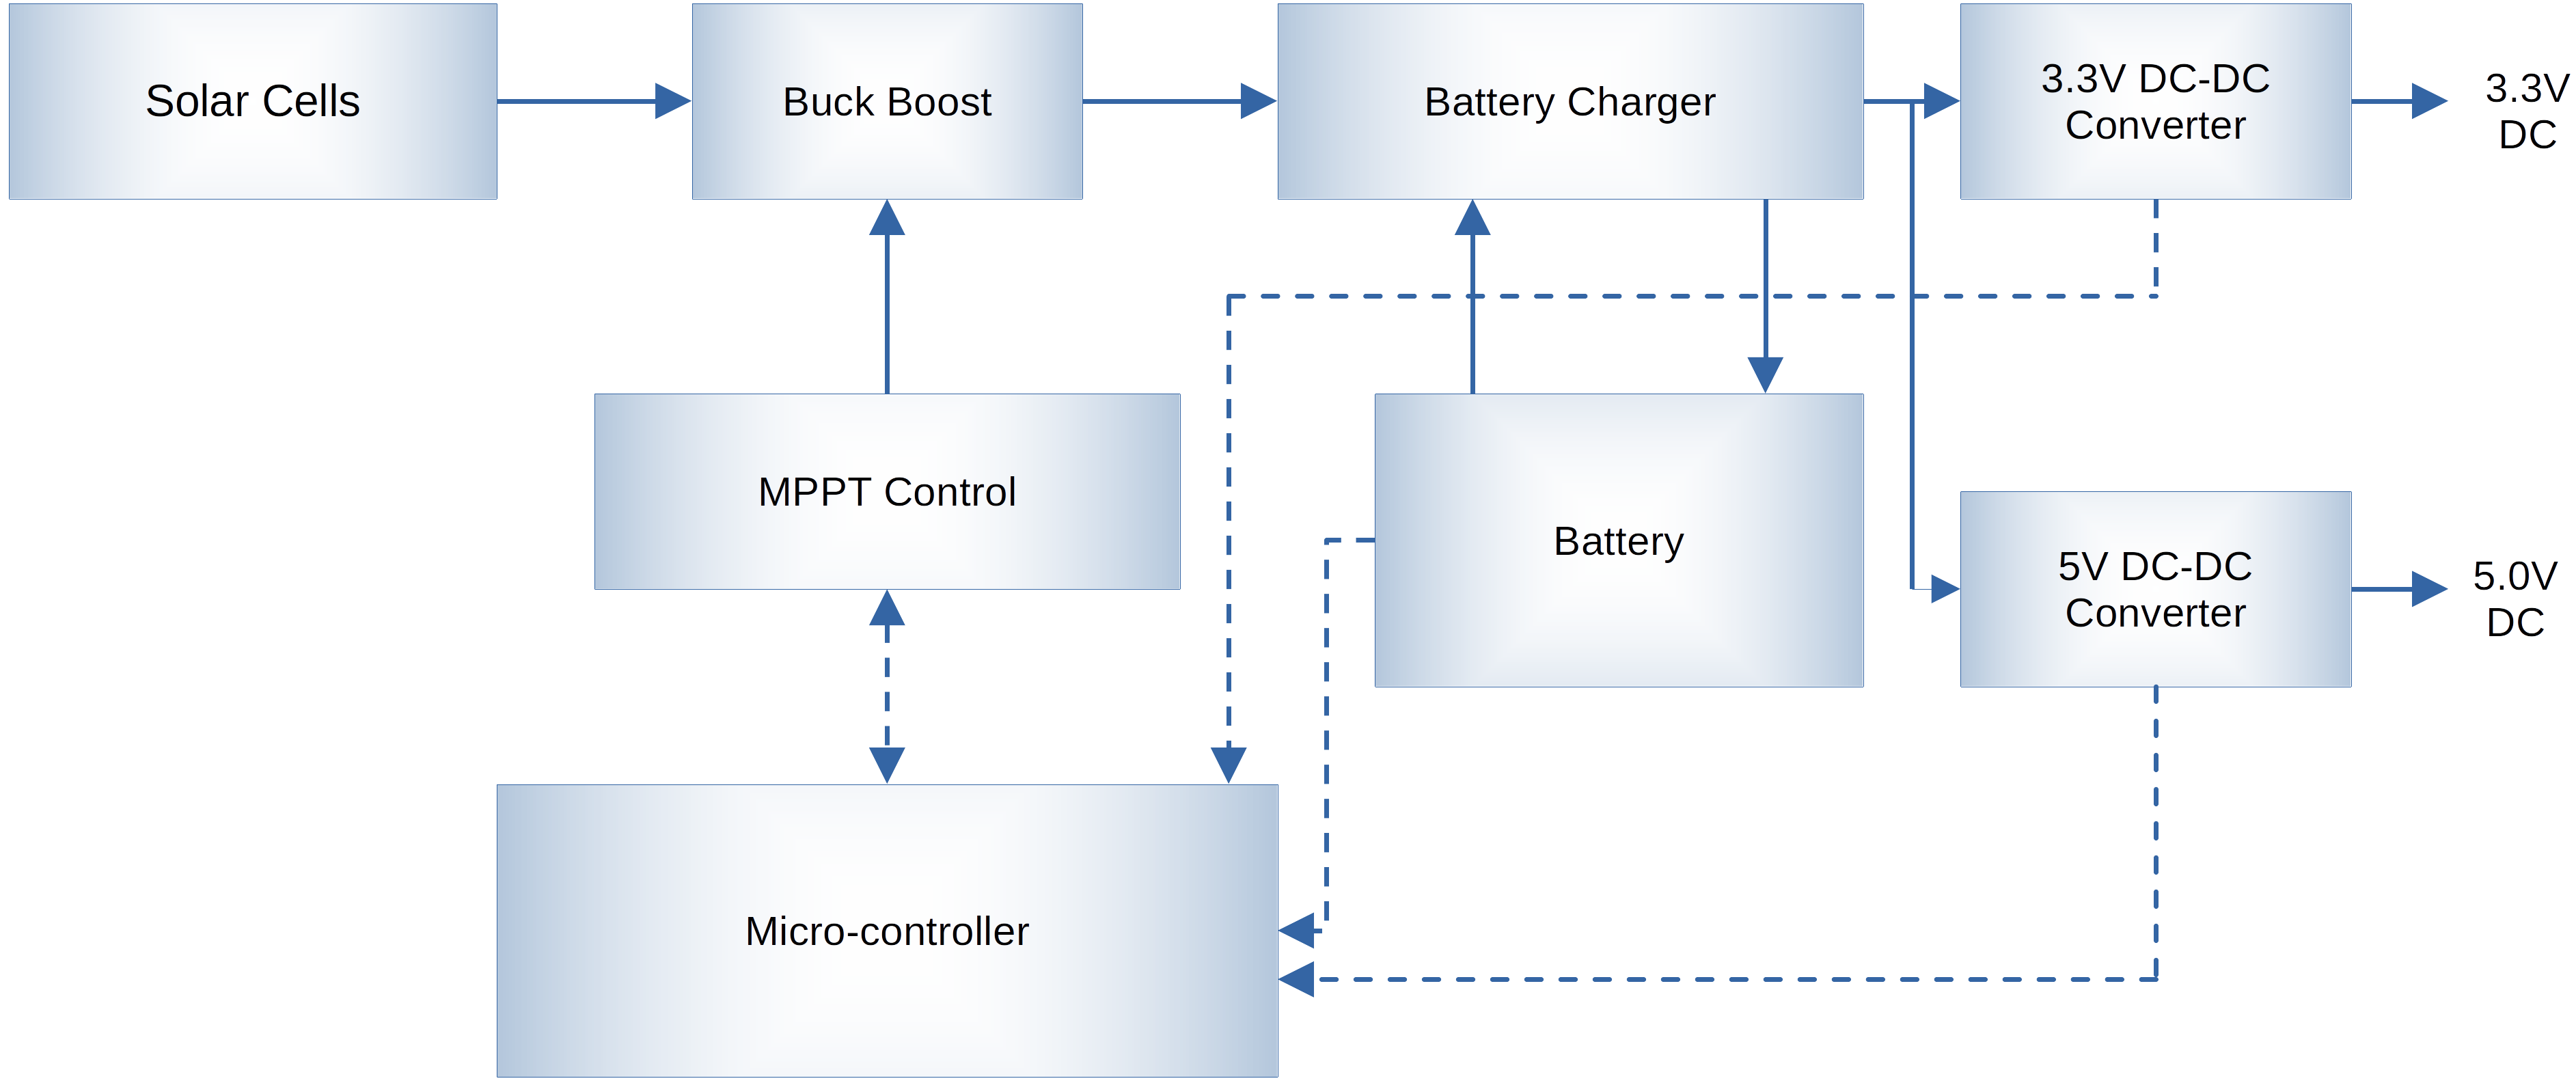
\includegraphics[width=0.9\textwidth]{blk diag.png}
			\caption{CubeSat EPS Architecture}
			\label{fig:mesh1}
		\end{figure}
		
		
	\end{frame}
	
	\section{Methodology}
	
	
	
	
	
	
	\begin{frame}{Methodology}
		\begin{itemize}
			
			\item Identifying the power requirements
		\item Architecture design and topology selection
			\item Forming Specifications
			
			\item Design and simulation
			\item Procurement of components
			\item Fabrication and testing
			
		\end{itemize} 
		
	\end{frame}
	
	
	\section{Requirements}
	\begin{frame}{Requirements}
		\begin{minipage}{0.5\textwidth}
			Equipments Requirements:
			\begin{itemize}
				
				\item SMD Soldering Station
				\item Oscilloscope
				\item Power Supply
				\item Function Generator
			\end{itemize} 
		\end{minipage}
		\begin{minipage}{0.3\textwidth}
			Software Requirements:
			\begin{itemize}
				
				\item MATLAB/Spice
				\item KiCad
				\item STM32 CubeIDE
				
			\end{itemize} 
			
		\end{minipage}
	\end{frame}
	
	
	
	\section{Budget Estimate}
	\begin{frame}{Budget Estimate: Component cost}
		
		\begin{table}[]
			\begin{tabular}{|l|l|l|l}
				\cline{1-3}
				\textbf{Sl. No.} & \textbf{Item}                       & \textbf{Amount (Rs.)} &  \\ \cline{1-3}
				1                & STM32 NUCLEO Development Board      & 3000                  &  \\ \cline{1-3}
				2                & SMD soldering station               & 9000                  &  \\ \cline{1-3}
				3                & Li-ion Cell (x2)                  & 1000                  &  \\ \cline{1-3}
				4                & Regulated Multi-Output Power Supply & 5000                  &  \\ \cline{1-3}
				5                & Solar Panel                         & 2000                    &  \\ \cline{1-3}
				6                & Components                          & 8000         &  \\ \cline{1-3}
			\end{tabular}
		\end{table}
		
		
		
	\end{frame}
	
	
	\begin{frame}{Budget Estimate: Fabrication cost}
		\begin{table}[]
			\begin{tabular}{|l|l|l|l}
				\cline{1-3}
				\textbf{Sl. No.} & \textbf{Item}        & \textbf{Amount (Rs.)} &  \\ \cline{1-3}
				1                & PCB Printing         & 3000                    &  \\ \cline{1-3}
				2                & SMD soldering        & 990                    &  \\ \cline{1-3}
				3                & Inductor Fabrication & 1000                  &  \\ \cline{1-3}
			\end{tabular}
		\end{table}
	\end{frame}
	
	
	\section{Project Timeline}

	
	
	
	\begin{frame}{Project Timeline}
		
			\begin{figure}[h]
			\centering
			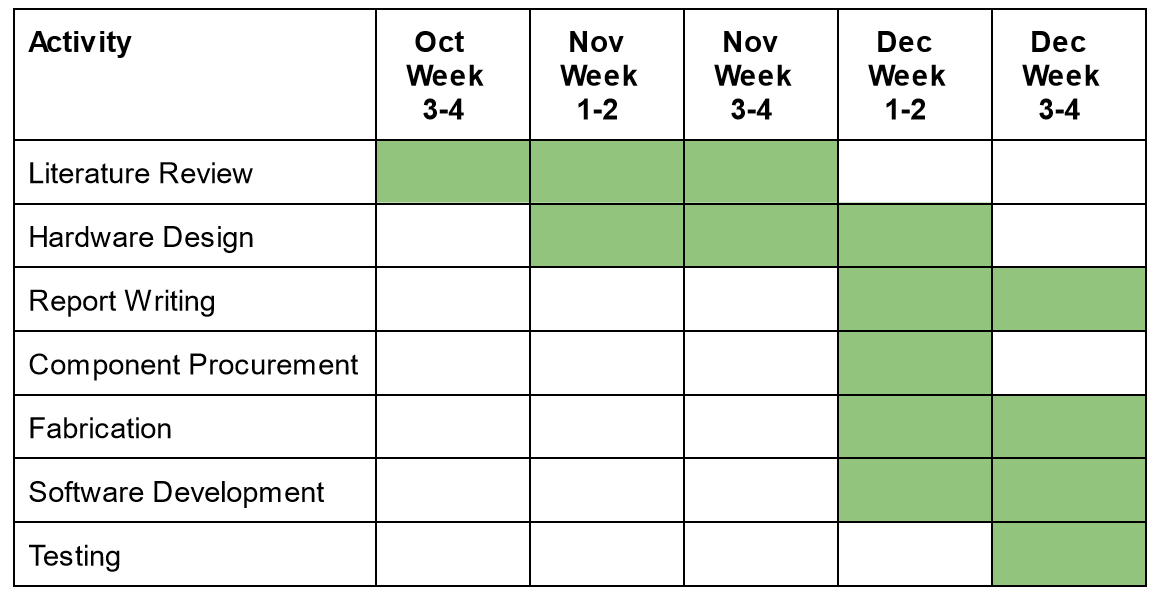
\includegraphics[width=0.9\textwidth]{tl.png}
%			\caption{CubeSat EPS Architecture}
			\label{fig:timel}
		\end{figure}

	\end{frame}
	
	
	\section{References}
	\begin{frame}[allowframebreaks]{References}
	
	\begin{thebibliography}{9}
			
					\bibitem[1]{p4}
		Knap, Vaclav \& Vestergaard, Lars \& Stroe, Daniel-Ioan (2020	)
		\newblock A Review of Battery Technology in CubeSats
		and Small Satellite Solutions
		\newblock \emph{Energies, vol. 13}	
				\bibitem[2]{p2}
			A. Edpuganti, V. Khadkikar, H. Zeineldin, M. S. E. Moursi and M. Al Hosani (2021)
			\newblock Comparison of Peak Power Tracking Based Electric Power System Architectures for CubeSats
			\newblock \emph{IEEE Transactions on Industry Applications, vol. 57, no. 3, pp. 2758-2768, May-June 2021}
			
		\bibitem[3]{p3}
		E. Ayoub and N. Karami 
		\newblock Review on the charging techniques of a Li-Ion battery
		\newblock \emph{Third International Conference on Technological Advances in Electrical, Electronics and Computer Engineering (TAEECE), 2015, pp. 50-55}
		
	
		
			\bibitem[4]{p1}
	B. Hussein, A. M. Massoud and T. Khattab (2022)
	\newblock Centralized, Distributed, and Module-Integrated Electric Power System Schemes in CubeSats: Performance Assessment
	\newblock \emph{ IEEE Access, vol. 10, pp. 55396-55407}
	
	






	\end{thebibliography}
	\end{frame}
	
	\begin{frame}
		
		
	\end{frame}
	%\end{frame}
\end{document} 